\documentclass[a4paper]{article}

\usepackage{graphicx}
\usepackage{amsmath,amssymb}
\usepackage{minted}
\usepackage{multirow}
\usepackage{float}
\usepackage{algorithm}
\usepackage{algpseudocode}
\usepackage{todonotes}
\usepackage{forest}
\usepackage{xstring}
\usepackage{xcolor}
\usepackage[most]{tcolorbox}
\usepackage{xparse}
\usepackage{natbib}
\usepackage{adjustbox}

\usetikzlibrary{graphs,graphdrawing}
\usegdlibrary{layered}

% for external graphviz
\input{/home/donkarlo/Dropbox/repo/nd_language_ai_project/src/nd_language_ai/formal/computer/programming/tex/latex/code_clips/external_graphviz.tex}

% for tags
\input{/home/donkarlo/Dropbox/repo/nd_language_ai_project/src/nd_language_ai/formal/computer/programming/tex/latex/part/control_sequence/kind/semtag/semtag.tex}

% for links
\input{/home/donkarlo/Dropbox/repo/nd_language_ai_project/src/nd_language_ai/formal/computer/programming/tex/latex/code_clips/seehere.tex}

% for nested lists and sections
\input{/home/donkarlo/Dropbox/repo/nd_language_ai_project/src/nd_language_ai/formal/computer/programming/tex/latex/code_clips/deep_structure.tex}

\title{}
\date{}
\author{Mohammad Rahmani}

\begin{document}

   \maketitle

   Dear Prof Rinner,

   I thought maybe because of you were busy you have forgotten about the documents that I sent you.
   Eventhough the solution is complete code wise but the I have been continousely working on  improving things both from architectural point and documenting it. I wanted to generate new documents for you but I am sure with a couple of git commands and using the tex editor I developed and watching github repository makes continuous supervison easy and heart warming for me.

   I am sure if I explain you how things work in a meeting,you will be happy the extent of the work I have covered. It is inpired by neuroscience and linguics for the anomaly detection that unlike the previous paper it is used for autonomous navigation. That is when multiple robots are taught how to do something, then what ever throws them out of what they learned as normal cause them to think linguistically to reduce the anomaly and return back to equilibrium.

   I think this is a huge leap and long time ago I could do only anomally detection with LSTMs, but I really wanted to give the sense of thinking to multiple robots by imitating neurology.

   I want to draw your attention to the fact that I worked hard to acomplish this. Everyday after work I have worked multiple hours on it. In last three years I didnt visited my country to be able to use my vacation time to work on this. So a little encouragement from you would be nice. For example: I was chedcking github log for the python repositories that I sent in previous documents and I found currently I have created 1862 python files and I saved the changes (committed) them more 399 times. Just for the autonomous navigation that I sent the video, pycharm shows 38 files (imagine them as gears) work together. Higher number of files shows how modular and with care I have devlopped the code.

   On theother hand, to have a better understanding how much I read and took notes to be abale toi connect the points in my mind, a log from github shows me I have read about 591 topics and I saved the history over 161 times.

   I have made the the repositories available to you many times. But the in my previous email, I sent a specific document for it.

   Please not that these are only new repositories that I created in 1.5 years ago, but its four years I have this idea to imitate a neuron for novelty detection and autonomous navigation and I have those repositories on git hub too.

   I would really pay attention to my efforts as when I joined you I knew nothing about robotics but I had to accomplish this I had learn and take notes from control theory to neuroscience.

   It would be nice of you if you introduce me a journal of your choice so that I can organize the results in it. journal\_2026.pdf was supposed to be a journal, but it turned out to be the basis of my thesis. I ddint want it to be so long, but I wanted it to include all the details. It was a thinking pad that turned out to be an organised base for my thesis. I am improving it almost everyday.

   In recent days I have searcehd for more rlevant journals. It would be nice if you either pickone or introduce me one of your preference. Doesnt matter how hard the acceptance is. I look for no shortcuts. I will improve it so much that finally get accepted. I tried my best to consider the NES list for publication quality and also the relevance in my mind. I believe this new list is better.  Knowing in which journal to publish is like a light that shows the way. In journal\_2026.pdf, I was only trying to novelty detection success, but there are a lot of figures and numbers that can be drawn out of the code. I just need to know journal limitations. I will add imporatnt results gradually to current document.


   \textbf{Manuscript:} Self-awareness in Multi-Robot Systems.

   \textbf{NES criterion:} Category I requires Q1 in at least one
   Scimago subject category in one of the preceding two years.
   Q2 and Q3 journals belong to Category II.

      \subsection{Recommended Journals}


   \section{Potential Journals for Neurorobotics-Related Papers}

      \begingroup
      \scriptsize
      \renewcommand{\arraystretch}{1.2}
      \setlength{\tabcolsep}{4pt}


      \begin{table}[p]
         \centering

         \caption{Potential journals for Self-awareness in Multi-Robot Systems}
         \label{tab:neurorobotics_journals}

         \begin{tabular}{@{}p{0.29\textwidth}p{0.08\textwidth}p{0.08\textwidth}p{0.43\textwidth}@{}}
\hline
\textbf{Journal} & \textbf{SJR} & \textbf{NES} & \textbf{Suitability for the paper} \\
\hline
\href{https://cis.ieee.org/publications/t-cognitive-and-developmental-systems}{IEEE Transactions on Cognitive and Developmental Systems} & Q1 & I & Very high. Cognitive architectures, developmental learning, and brain-inspired robotic cognition. \\
\hline
\href{https://www.keaipublishing.com/en/journals/cognitive-robotics/}{Cognitive Robotics} & Q1 & I & Very high. Cognitive processes, robotic learning, and sensory-to-language representation learning. \\
\hline
\href{https://link.springer.com/journal/10514}{Autonomous Robots} & Q1 & I & High. Robotic learning, perception, autonomy, and adaptive behavior. \\
\hline
\href{https://www.sciencedirect.com/journal/robotics-and-autonomous-systems}{Robotics and Autonomous Systems} & Q1 & I & High. Cognitive architectures demonstrated through autonomous navigation and multi-robot experiments. \\
\hline
\href{https://journals.sagepub.com/home/adb}{Adaptive Behavior} & Q1 & I & High. Biologically inspired adaptive behavior, cognitive mechanisms, and regulation. \\
\hline
\href{https://www.sciencedirect.com/journal/neural-networks}{Neural Networks} & Q1 & I & Suitable if the primary novelty is the neural learning or representation algorithm. \\
\hline
\href{https://link.springer.com/journal/12369}{International Journal of Social Robotics} & Q1 & I & Suitable if robot--robot communication and self--other distinction are central contributions. \\
\hline
\href{https://direct.mit.edu/neco}{Neural Computation} & Q1 & I & Suitable if the primary contribution is the computational or theoretical neural model. \\
\hline
\href{https://www.frontiersin.org/journals/neurorobotics}{Frontiers in Neurorobotics} & Q2 & II & Very high topical fit. Neurally inspired autonomous systems, embodied cognition, and neural control. \\
\hline
\href{https://www.sciencedirect.com/journal/cognitive-systems-research}{Cognitive Systems Research} & Q2 & II & Very suitable for cognitive architectures and theoretical models of artificial cognition. \\
\hline
\href{https://www.ieee-ras.org/publications/ra-l/}{IEEE Robotics and Automation Letters} & Q1 & I & Suitable for a focused robotics contribution supported by strong empirical results. \\
\hline
\href{https://iopscience.iop.org/journal/1748-3190}{Bioinspiration \& Biomimetics} & Q1 (2024) & I & Suitable if biological inspiration is explicitly formalized and empirically validated. \\
\hline
\href{https://www.ieee-ras.org/publications/t-ro/}{IEEE Transactions on Robotics} & Q1 & I & Suitable for substantial robotics novelty supported by strong experimental validation. \\
\hline
\href{https://www.science.org/journal/scirobotics}{Science Robotics} & Q1 & I & Suitable for an exceptional, broadly significant robotics contribution with convincing experimental evidence. \\
\hline
\end{tabular}

      \end{table}

      \endgroup





\begin{itemize}
    \item Private meetings with Rinner. some days ago I search for it but it was not in course lists, now it is  but it says it is too late. What should I do? \begin{figure}[H] \centering 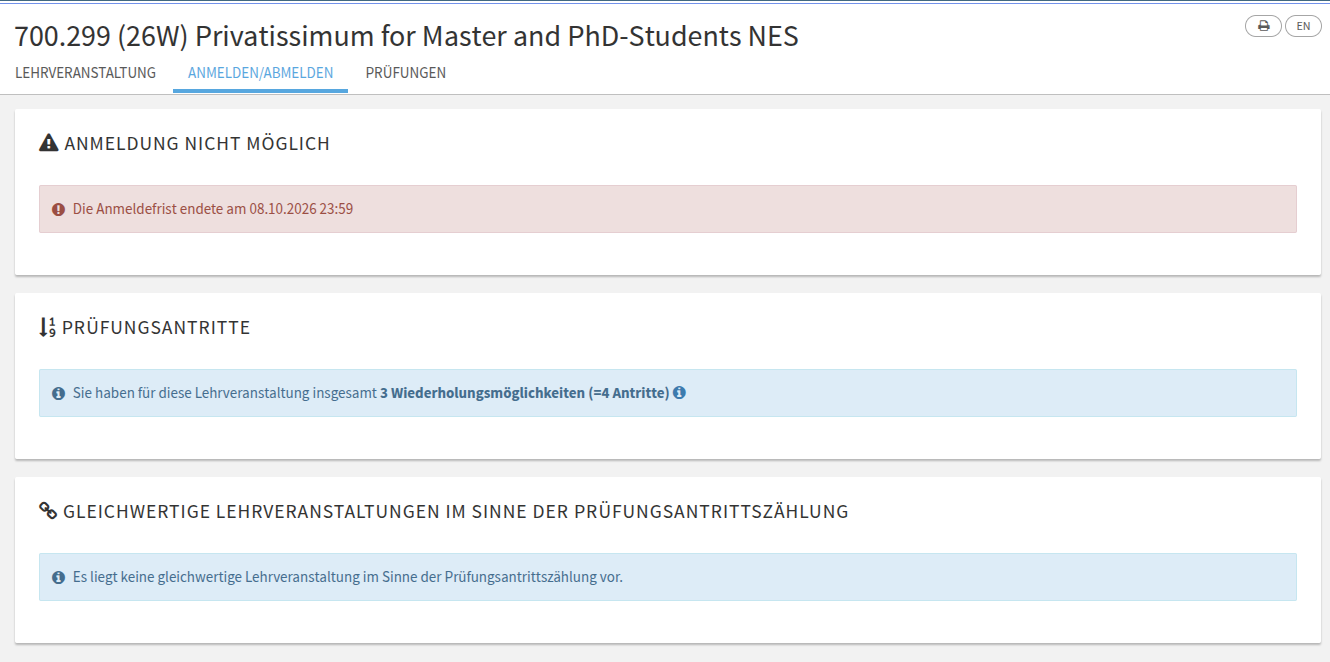
\includegraphics[width=0.9\textwidth]{private_meeting.png} \end{figure}
\end{itemize}
      \bibliographystyle{plainnat}
      \bibliography{/home/donkarlo/Dropbox/repo/nd_shared_research/bibliography/bibliography.bib}

\end{document}
